%
% $RCSfile: introduction.tex,v $
%
% Copyright (C) 2002-2008. Christian Heller.
%
% Permission is granted to copy, distribute and/or modify this document
% under the terms of the GNU Free Documentation License, Version 1.1 or
% any later version published by the Free Software Foundation; with no
% Invariant Sections, with no Front-Cover Texts and with no Back-Cover
% Texts. A copy of the license is included in the section entitled
% "GNU Free Documentation License".
%
% http://www.cybop.net
% - Cybernetics Oriented Programming -
%
% http://www.resmedicinae.org
% - Information in Medicine -
%
% Version: $Revision: 1.1 $ $Date: 2008-08-19 20:41:07 $ $Author: christian $
% Authors: Christian Heller <christian.heller@tuxtax.de>
%

\chapter{Introduction}
\label{introduction_heading}
\index{Introduction}
\index{Information Technology}
\index{Information Age}
\index{Information}
\index{Software}

\begin{flushright}
    \textsl{Even a Way of a thousand Miles begins with one Step.}\\
    \textsc{Saying}
\end{flushright}

\emph{Information Technology} is gaining more and more importance in modern
society. Some people even talk of the \emph{Information Age}. What
\emph{Electricity} was for the \emph{Industrial Age}, \emph{Information} is for
today's society.

And \emph{Software} plays one of the, if not the most important role thereby.

%
% $RCSfile: information_science.tex,v $
%
% Copyright (C) 2002-2008. Christian Heller.
%
% Permission is granted to copy, distribute and/or modify this document
% under the terms of the GNU Free Documentation License, Version 1.1 or
% any later version published by the Free Software Foundation; with no
% Invariant Sections, with no Front-Cover Texts and with no Back-Cover
% Texts. A copy of the license is included in the section entitled
% "GNU Free Documentation License".
%
% http://www.cybop.net
% - Cybernetics Oriented Programming -
%
% http://www.resmedicinae.org
% - Information in Medicine -
%
% Version: $Revision: 1.1 $ $Date: 2008-08-19 20:41:07 $ $Author: christian $
% Authors: Christian Heller <christian.heller@tuxtax.de>
%

\section{Information Science}
\label{information_science_heading}
\index{Information Science}
\index{Scientific Inventions}
\index{Robot}
\index{Computer}
\index{Hardware}
\index{Software}
\index{Informatics}
\index{Abstract Model}

\emph{Science} is one form in which humans express their aspiration for
\emph{Perception}. It should -- but unfortunately not always does -- serve the
well-being of people. Similarly, scientific \emph{Inventions} usually are to
ease human's life.

\begin{figure}[ht]
    \begin{center}
        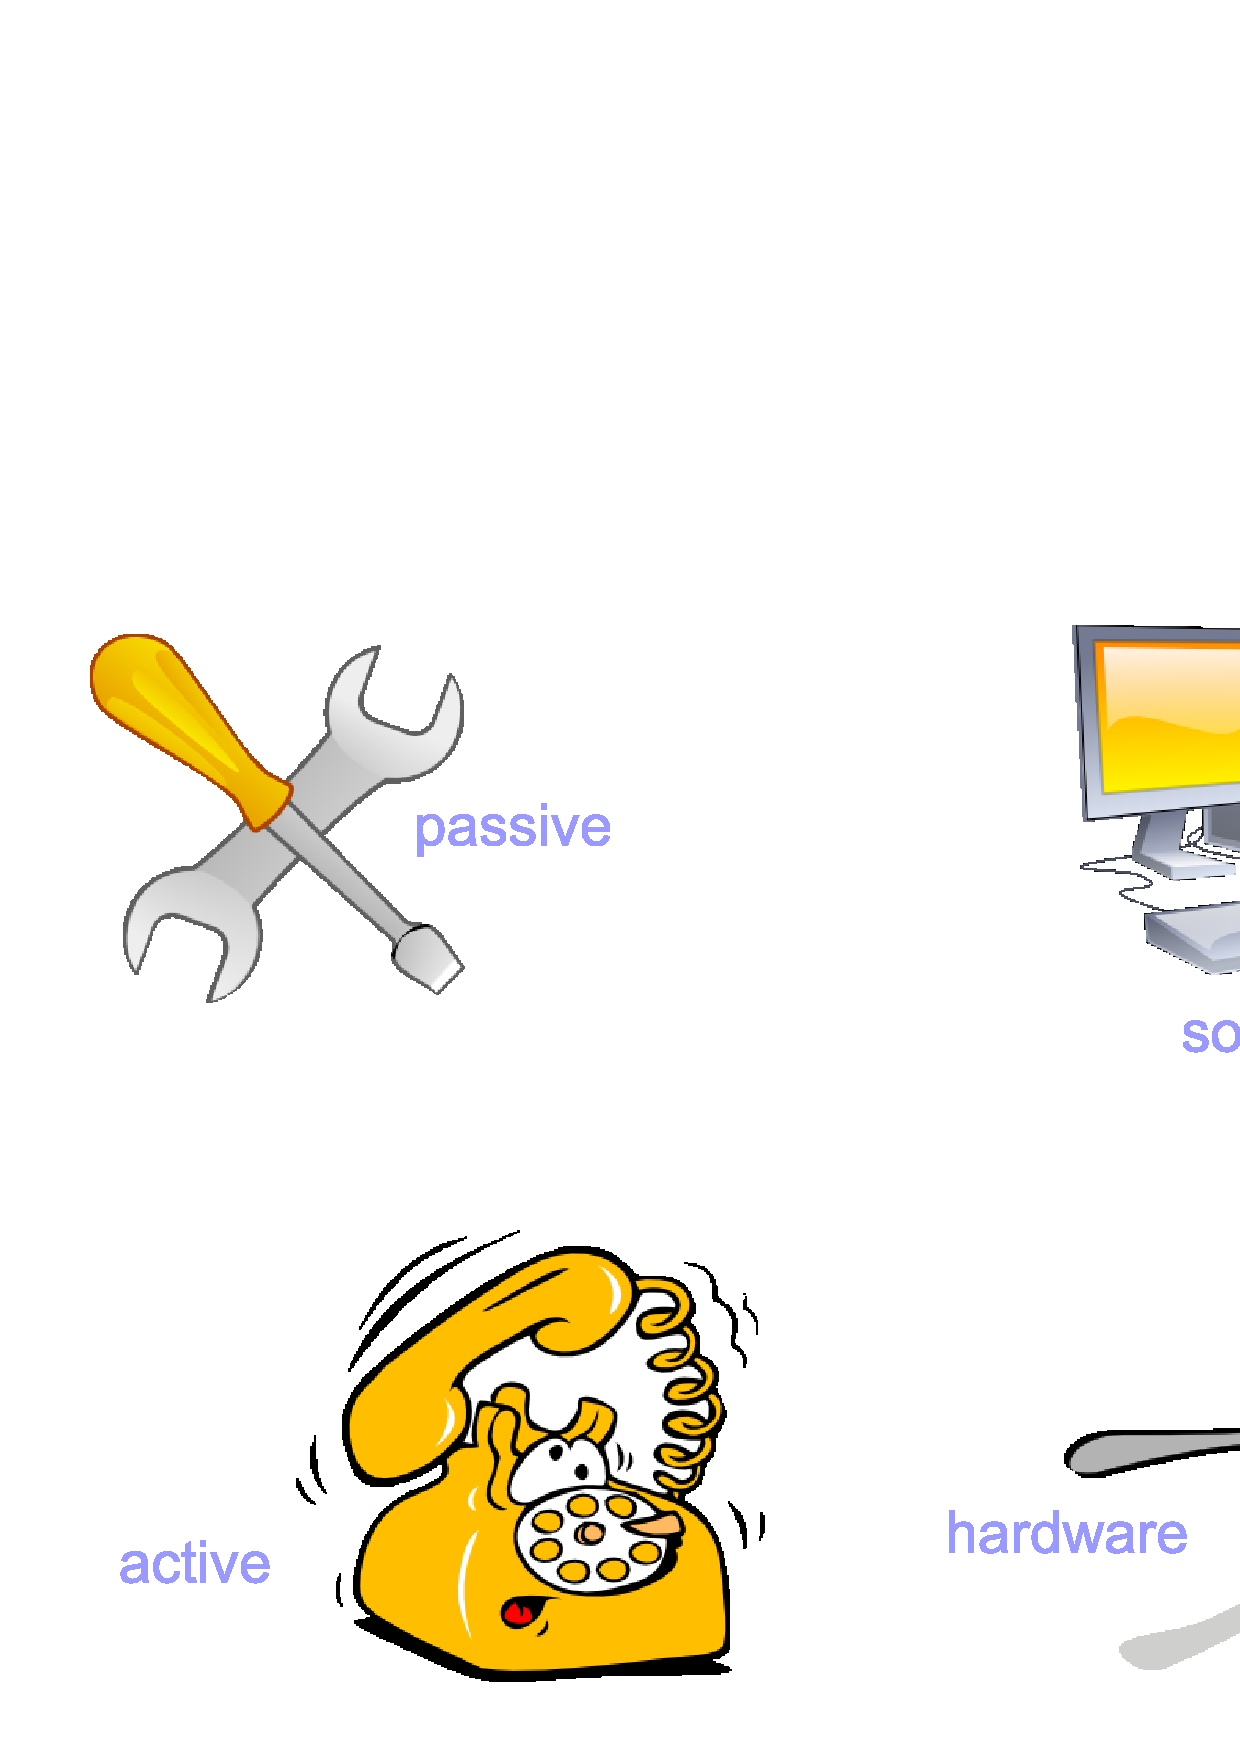
\includegraphics[scale=0.3,angle=-90]{graphic/inventions.pdf}
        \caption{Scientific Inventions}
        \label{inventions_figure}
    \end{center}
\end{figure}

The results of many technical inventions are \emph{Tools}, \emph{Machines} or
\emph{Robots} (figure \ref{inventions_figure}). A passive tool is a mostly
simple device used by humans to carry out a task better. The word machine is
used to describe advanced, active tools which can run by themselves, only
driven by an external force like steam or electrical energy. A robot, finally,
is an enhanced machine which may imitate human behaviour (humanoid) or take
over (industrial) tasks that are too dirty, dangerous, difficult, repetitive or
dull for humans \cite{wikipedia}. Its parts are often called \emph{Hardware}.
It does not necessarily have the same shape as the human body but can come very
close. Also, it contains some pieces of rudimentary \emph{Intelligence} that
lets it act alone (autonomous). The intelligence basically controls the way in
which the robot functions what is sometimes called \emph{Workflow} or
\emph{Program}. That must be encoded, for example in form of a \emph{Punchcard}
or pieces of \emph{Software}, kept as pure text or binary data in some
electronic memory or on a storage medium.

A \emph{Computer} can be seen as handicaped robot that can think but not move.
Essentially, it represents the intelligent parts of a robot and is able to
process (\emph{compute}) \emph{Information} (data content of a message
\cite{duden}). But its hardware is pruned to pure information input and output.
While the importance of robots lies in their \emph{Movement} actions, it lies
in problem \emph{Solving} and system \emph{Simulation} for computers
\cite{wikipedia}. Software plays the biggest role thereby. It contains the
programs after which a computer is run, after which it acts.

One important area the science of information, called \emph{Informatics}, deals
with is software -- the art of \emph{representing} and \emph{processing}
information. As such, one of its major aims is to find \emph{Abstract Models}
which represent the real world best. The better this is done and the better
information can be stored and processed, the better software can assist its
human users.

%
% $RCSfile$
%
% Copyright (c) 2002-2006. Christian Heller. All rights reserved.
%
% Permission is granted to copy, distribute and/or modify this document
% under the terms of the GNU Free Documentation License, Version 1.1 or
% any later version published by the Free Software Foundation; with no
% Invariant Sections, with no Front-Cover Texts and with no Back-Cover
% Texts. A copy of the license is included in the section entitled
% "GNU Free Documentation License".
%
% http://www.cybop.net
% - Cybernetics Oriented Programming -
%
% http://www.resmedicinae.org
% - Information in Medicine -
%
% Version: $Revision$ $Date$ $Author$
% Authors: Christian Heller <christian.heller@tuxtax.de>
%

\subsection{Software Crisis}
\label{software_crisis_heading}

An early question in software engineering was how to write programs that control
a computer system's \emph{Hardware} correctly and efficiently. Over time, the
importance of hardware shifted in favour of \emph{Software} which nowadays
contains most of the logic needed to run an application on a computer system.
Consequently, much more research emphasis is now placed on the finding of clever
modelling concepts that help writing correct and effective, stable and robust,
flexible and maintainable, secure software. Another objective is to increase the
effectiveness and lessen the expenditure of cost and time in software development
projects, by \emph{reusing} (pieces of) software.

The past 40 years have delivered numerous helpful concepts, for instance
\emph{Structure} and \emph{Procedure}, \emph{Class} and \emph{Inheritance},
\emph{Pattern} and \emph{Framework}, \emph{Component} and \emph{Concern}, and
many more. They undoubtedly have moved software design far forward. Nevertheless,
the dream of true componentisation and full reusability has not been reached.
Czarnecki \cite{czarnecki} identifies problems in the four areas: \emph{Reuse},
\emph{Adaptability} (\emph{Flexibility}), management of \emph{Complexity} and
\emph{Performance}.

Modern software is very \emph{complex}. It runs on different hardware platforms,
uses multiple communication paradigms and offers various user interfaces. Many
tools and methods assist experts as well as engineers in creating and maintaining
software but do they not seem sufficient to cope with the complexity so that
often, systems still base on buggy source code causing:

\begin{itemize}
    \item[-] False Results
    \item[-] Memory Leaks
    \item[-] Endless Loops
    \item[-] Weak Performance
    \item[-] Security Holes
\end{itemize}

Are these exclusively the fault of software developers? Or, are the used
concepts perhaps insufficient? Using the same, allegedly unsatisfying concepts
caused some people to talk about an ongoing \emph{Software Crisis}, sometimes
\emph{Complexity Crisis}, affecting not only high-level application programming,
but also low-level microchip design \cite{daene}.

However, answers are not easy to find. Software design is \emph{Arts} and
\emph{Engineering}, at the same time. Not everything is or can be regulated by
rules. It is true, developers have to stick to a set of design rules -- and
tools that support their usage exist -- but they also have to be very creative.
All the time, they have to have new, innovative ideas and apply them to software.
This is what makes the creation, integration, test and maintenance of software
so difficult. There is not really a uniform way of treating it.

%
% $RCSfile: motivation.tex,v $
%
% Copyright (C) 2002-2008. Christian Heller.
%
% Permission is granted to copy, distribute and/or modify this document
% under the terms of the GNU Free Documentation License, Version 1.1 or
% any later version published by the Free Software Foundation; with no
% Invariant Sections, with no Front-Cover Texts and with no Back-Cover
% Texts. A copy of the license is included in the section entitled
% "GNU Free Documentation License".
%
% http://www.cybop.net
% - Cybernetics Oriented Programming -
%
% http://www.resmedicinae.org
% - Information in Medicine -
%
% Version: $Revision: 1.1 $ $Date: 2008-08-19 20:41:07 $ $Author: christian $
% Authors: Christian Heller <christian.heller@tuxtax.de>
%

\section{Motivation}
\label{motivation_heading}
\index{Motivation}
\index{Abstraction Gaps}
\index{Misleading Tiers}
\index{Modelling Mistakes}
\index{Inter-Disciplinary Effort}

To the issues that this work has with some state-of-the-art solutions belong in
particular three things:

\begin{enumerate}
    \item \emph{Abstraction Gaps} in Software Engineering Process (chapter
        \ref{software_engineering_process_heading})
    \item \emph{Misleading Tiers} in Physical Architecture (chapter
        \ref{physical_architecture_heading})
    \item \emph{Modelling Mistakes} in Logical Architecture (chapter
        \ref{logical_architecture_heading})
\end{enumerate}

The traversing of abstraction gaps in a software engineering process belongs to
the main difficulties in software development, and causes considerable cost-
and time effort. It necessitates a steady synchronisation between domain
experts and application system developers, because their responsibilities
cannot be clearly separated and interests often clash. A first objective of
this work is therefore to contribute to closing these gaps, especially the one
existing between a designed system architecture and the implemented source
code.

The misinterpretation of the physical tiers in an information technology
environment often leads to wrong-designed software architectures. Logical
layers are adapted to physical tiers (frontend, business logic and backend) and
differing patterns are used to implement them. Instead, systems should be
designed in a way that allows the usage of a unified translator architecture,
so to give every application system the capability to communicate universally
by default, which is the second objective of this work.

Several well-known issues exist with the modelling of logical system
architectures, for example: fragile base class problem, container inheritance,
bidirectional dependencies, global data access. These and others more result
from using wrong principles of knowledge abstraction, like the bundling of
attributes and methods in one class, as suggested by object oriented
programming, or the equalising of structural- and meta information in a model.
A third and final aim of this work is therefore to closer investigate the basic
principles and concepts after which current software systems are created, and
to search for new ideas and concepts, with the objective of finding a universal
type structure (knowledge schema).

On its search for new ideas, this work intentionally tries to cross the borders
to other scientific disciplines. It can therefore also be called an
\emph{inter-disciplinary} effort. Results from many different sciences are
applied to software engineering. Most emphasis, however, is placed on the
comparison between human- and computer systems. Nature has always been a good
teacher and its principles have often been copied; so does this work.

%
% $RCSfile: cybernetics.tex,v $
%
% Copyright (C) 2002-2008. Christian Heller.
%
% Permission is granted to copy, distribute and/or modify this document
% under the terms of the GNU Free Documentation License, Version 1.1 or
% any later version published by the Free Software Foundation; with no
% Invariant Sections, with no Front-Cover Texts and with no Back-Cover
% Texts. A copy of the license is included in the section entitled
% "GNU Free Documentation License".
%
% http://www.cybop.net
% - Cybernetics Oriented Programming -
%
% http://www.resmedicinae.org
% - Information in Medicine -
%
% Version: $Revision: 1.1 $ $Date: 2008-08-19 20:41:06 $ $Author: christian $
% Authors: Christian Heller <christian.heller@tuxtax.de>
%

\section{Cybernetics}
\label{cybernetics_heading}
\index{Cybernetics}
\index{Kybernetes}
\index{Bionics}
\index{Bio-Cybernetics}
\index{Software Engineering}
\index{Systems Engineering}
\index{Cybernetics Oriented Programming}
\index{CYBOP}

One scientific subject being inter-disciplinary since its creation is
\emph{Cybernetics}. Its name stems from the ancient Greek word \emph{Kybernetes}
meaning \emph{Steersman} and it has many definitions \cite{heylighen}. One that
was coined in 1948 by \emph{Norbert Wiener} sees \emph{Cybernetics} as the
science of information and control, no matter whether it is about living things
or machines. The \emph{American Heritage Dictionary of the English Language}
\cite{americanheritagedictionary} defines it as \textit{the theoretical study
of communication and control processes in biological, mechanical, and electronic
systems, especially the comparison of these processes in biological and
artificial systems}.

The closely related subject of \emph{Bionics} is a specialisation of cybernetics
(\emph{Bionics} = \emph{Bio-Cybernetics}) \cite{designmatrix}. It can be defined
as the \textit{application of biological principles to the study and design of
engineering systems} \cite{americanheritagedictionary}.

Other related fields which are not considered further in this work are morphology
(structure-function), general systems theory (complexity, isomorphic relationships),
biomechanics (prosthetics), biomimetics, robotics and artificial intelligence.
However, the results described in this document might also be of importance in
those areas.

Since \emph{Software Engineering} is a kind of \emph{Systems Engineering}, the
consideration of systems as a whole gains in importance. \emph{Cybernetics} as
science of observing, comparing and controlling biological and technical systems
is of great importance in the document on hand. Using models inspired by biology
and psychology (but also further disciplines such as philosophy or physics), the
science of \emph{Bionics} plays an important role, too.

Sticking to the system idea of \emph{Wiener} and in the fashion of the science
of \emph{Bionics}, this work and the new concepts described therein are called
\emph{Cybernetics Oriented Programming} (CYBOP).

%
% $RCSfile$
%
% Copyright (c) 2005-2006. Christian Heller. All rights reserved.
%
% Permission is granted to copy, distribute and/or modify this document
% under the terms of the GNU Free Documentation License, Version 1.1 or
% any later version published by the Free Software Foundation; with no
% Invariant Sections, with no Front-Cover Texts and with no Back-Cover
% Texts. A copy of the license is included in the section entitled
% "GNU Free Documentation License".
%
% http://www.cybop.net
% - Cybernetics Oriented Programming -
%
% http://www.resmedicinae.org
% - Information in Medicine -
%
% Version: $Revision$ $Date$ $Author$
% Authors: Christian Heller <christian.heller@tuxtax.de>
%

\subsection{Method}
\label{method_heading}

The work described in this article was undertaken in form of
\emph{Constructive Development}, as method of research. That is, an application
prototype \emph{Res Medicinae} (section \ref{res_medicinae_heading}) for use in
the medical domain was developed in parallel to the actual theoretical
investigations.

Prototype development started off by creating a state-of-the-art software
architecture using \emph{Object Oriented Programming} (OOP) principles and the
\emph{Java} programming language. When the first design problems occured, these
were solved by applying suitable software patterns -- mainly those of
\cite{gamma1995,buschmann,fowler2002}. The steady search for a flexible
architecture with only few dependencies then lead to the restructuring of the
application prototype, according to the recommendations of
\emph{Component Oriented Programming} (COP) with \emph{Concern Interfaces}, as
suggested at that time by the \emph{Apache-Jakarta-Avalon} project \cite{avalon}.

\begin{figure}[ht]
    \begin{center}
        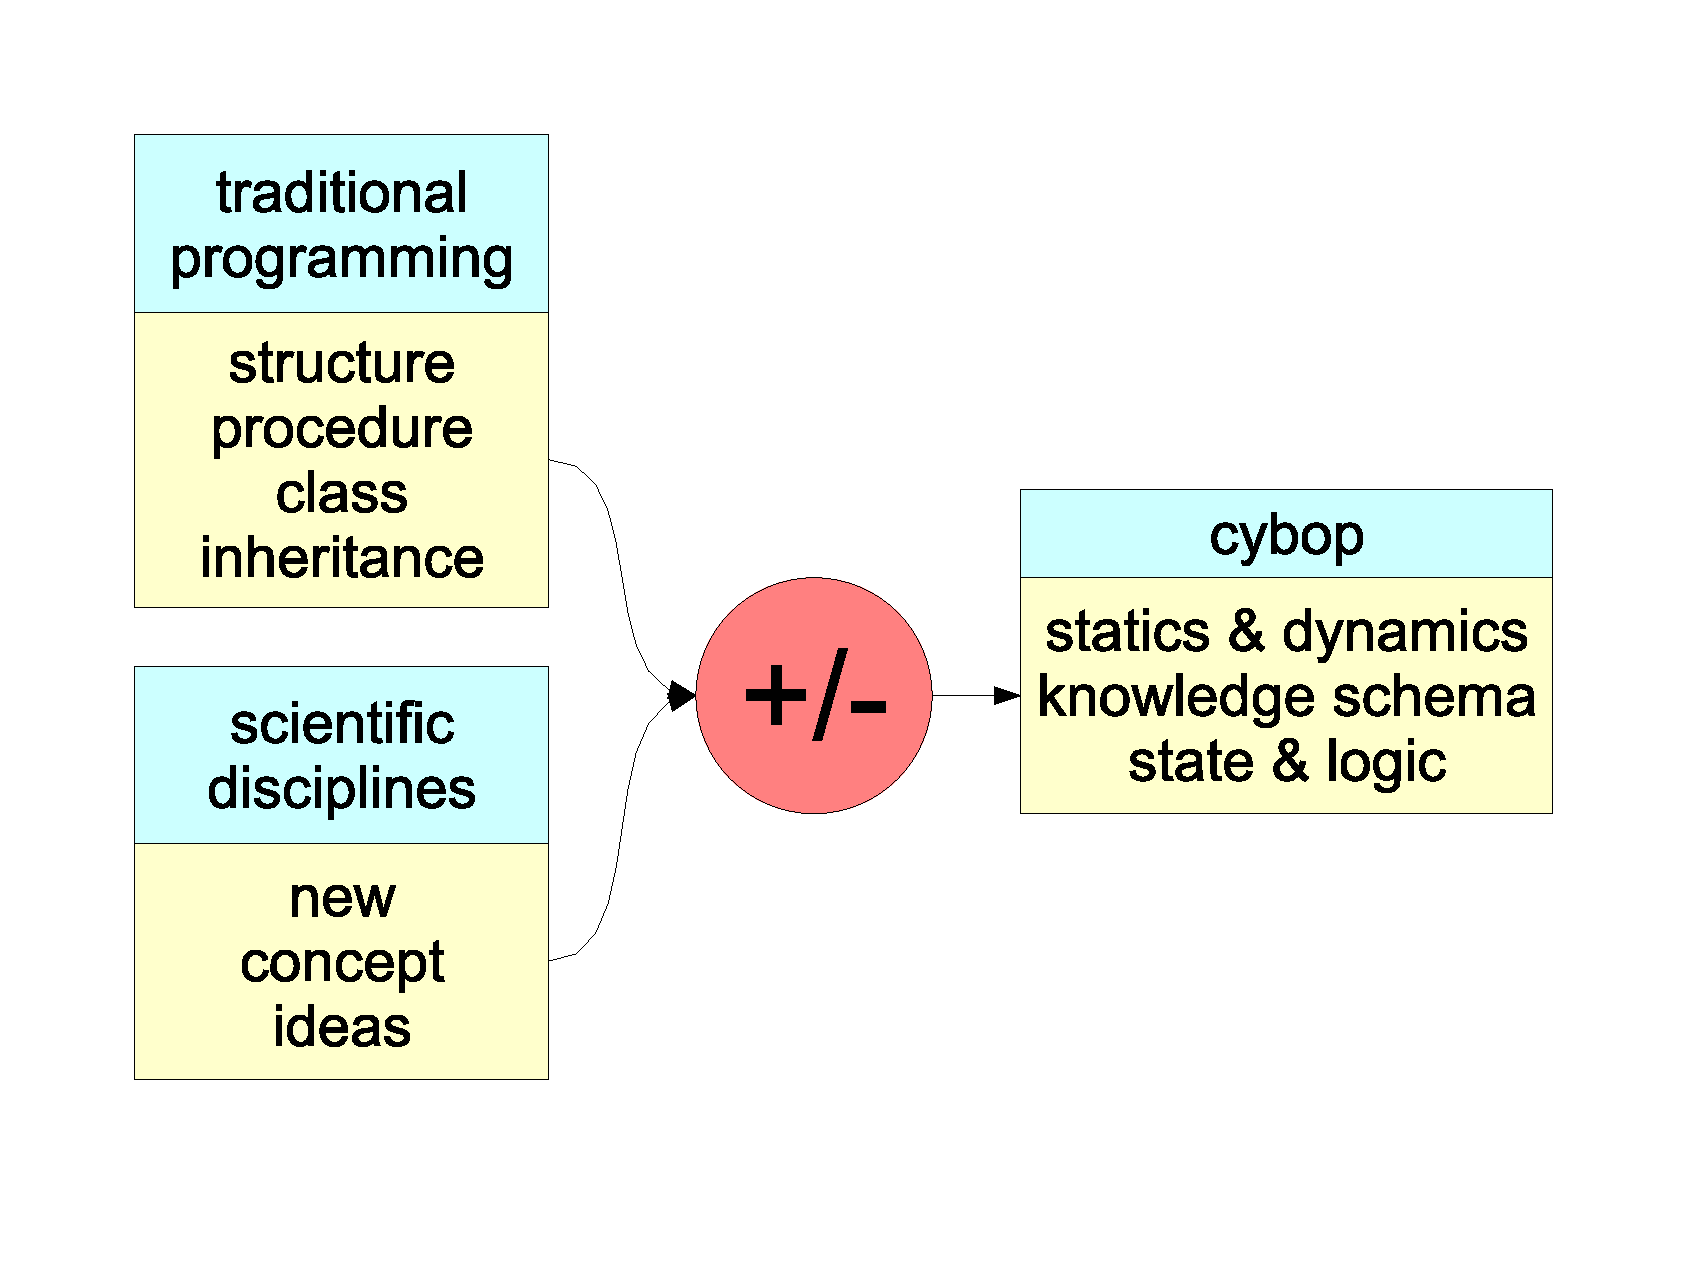
\includegraphics[scale=0.2]{vector/method.eps}
        \caption{Merger of Concepts}
        \label{method_figure}
    \end{center}
\end{figure}

However, these refactorings were only some of at least two dozens, since also
COP and the application of concerns, as well as other concepts applied later
(e.g. ontological structure implemented using the means of OOP) turned out to
have their deficiencies. According to the idea mentioned before, traditional
concepts were thus complemented, merged or revised with new concepts stemming
from other scientific disciplines (figure \ref{method_figure}), whenever a
classical design solution became unsatisfying.

Over the creation of a framework called \emph{ResMedLib}, which encapsulated
general application functionality, the prototype development finally ended up
in a complete reengineering: most of the functionality formerly residing in the
framework was moved into an interpreter (section \ref{cyboi_heading}) written
in the \emph{C} programming language; the actual application knowledge, on the
other hand, was put into special files, for which an
\emph{Extensible Markup Language} (XML)-based language (section
\ref{cybol_heading}) was defined.

Since problems did not occur in a predictable way, while developing the
mentioned prototype application, their presentation in order of appearance
would be rather confusing. An adapted structure of sections is therefore used
in this article, which first describes a number of observed discrepancies
(section \ref{existing_problems_heading}), then reflects on the most essential
new concepts (section \ref{reflexions_on_concepts_heading}), before it later
explains how these were implemented in practice (section
\ref{practical_proof_heading}).

%
% $RCSfile: example.tex,v $
%
% Copyright (c) 2001-2004. Christian Heller. All rights reserved.
%
% No copying, altering, distribution or any other actions concerning this
% document, except after explicit permission by the author!
% At some later point in time, this document is planned to be put under
% the GNU FDL license. For now, _everything_ is _restricted_ by the author.
%
% http://www.cybop.net
% - Cybernetics Oriented Programming -
%
% http://www.resmedicinae.org
% - Information in Medicine -
%
% @author Christian Heller <christian.heller@tuxtax.de>
%

\subsection{Example}
\label{example_heading}

The following example shows a minimalistic model of a (static) \emph{Graphical
User Interface} (GUI) frame.

\begin{verbatim}
<!--
    frame_example.cybol
/-->
<model>
    <part name="title"
        part_abstraction="string"
        part_model="Res Medicinae"/>
    <part name="menu_bar"
        part_abstraction="compound"
        part_model="/gui/menu_bar.cybol"
        position_abstraction="compass"
        position_model="north"/>
    <part name="status_bar"
        part_abstraction="compound"
        part_model="/gui/tool_bar.cybol"
        position_abstraction="compass"
        position_model="south"/>
</model>
\end{verbatim}

Similar models can be built of (dynamic) workflows whereby the inputs and outputs
of the part operations appear in a special order as attribute values. But this
may become the topic of a follow-up paper.

%
% $RCSfile: structure.tex,v $
%
% Copyright (C) 2002-2008. Christian Heller.
%
% Permission is granted to copy, distribute and/or modify this document
% under the terms of the GNU Free Documentation License, Version 1.1 or
% any later version published by the Free Software Foundation; with no
% Invariant Sections, with no Front-Cover Texts and with no Back-Cover
% Texts. A copy of the license is included in the section entitled
% "GNU Free Documentation License".
%
% http://www.cybop.net
% - Cybernetics Oriented Programming -
%
% http://www.resmedicinae.org
% - Information in Medicine -
%
% Version: $Revision: 1.1 $ $Date: 2008-08-19 20:41:09 $ $Author: christian $
% Authors: Christian Heller <christian.heller@tuxtax.de>
%

\section{Structure}
\label{structure_heading}
\index{Structure of this Book}

This document is divided into fourteen chapters. Neglecting this introduction,
thirteen chapters remain which are organised in four parts. They are illustrated
in figure \ref{structure_figure}.

\begin{figure}[ht]
    \begin{center}
        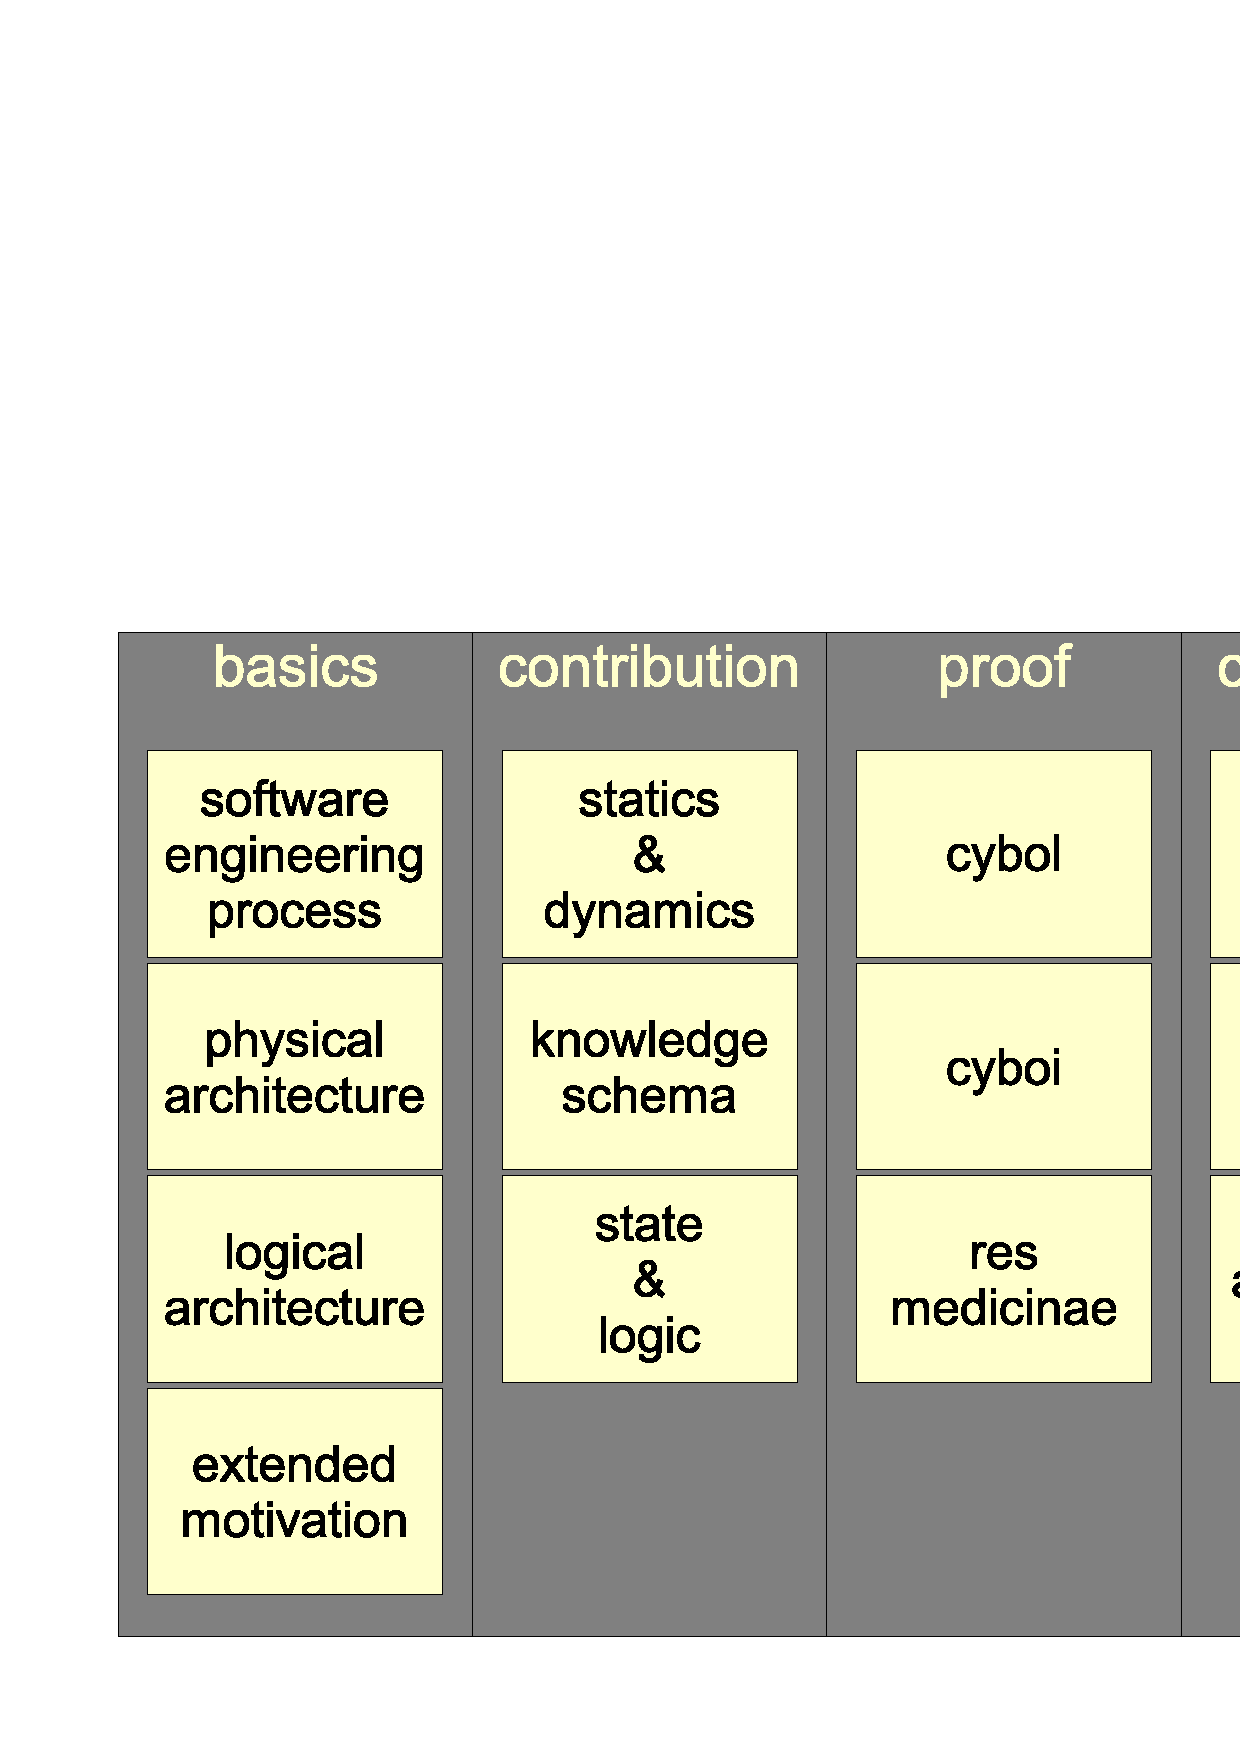
\includegraphics[scale=0.3,angle=-90]{graphic/structure.pdf}
        \caption{Document Structure}
        \label{structure_figure}
    \end{center}
\end{figure}

Part \ref{basics_heading} considers basic concepts of software development
(\emph{State of the Art}), before the then following part \ref{contribution_heading}
contributes new concept ideas. Practical proof of their operability is given in
part \ref{proof_heading}. And part \ref{completion_heading} finally completes
the work with a review, summary and outlook into the future.

\emph{Software Engineering Processes} (SEP) (chapter
\ref{software_engineering_process_heading}) have to be briefly described to be
able to estimate the effects of abstraction changes on the actual SEP phases.
The \emph{Physical Architecture} (chapter \ref{physical_architecture_heading})
of a standard \emph{Information Technology} (IT) environment is necessary
background knowledge for later reflections on the design of software systems
and their communication paradigms. Finally, the \emph{Logical Architecture}
(chapter \ref{logical_architecture_heading}), that is conceptual solutions for
structuring software systems, is investigated, to later be able to possibly
find \emph{Pros} and \emph{Cons}.

A short \emph{Recapitulation} of introduced state-of-the-art concepts and the
idea of an \emph{inter-disciplinary}, \emph{cybernetics-oriented} approach lead
to an \emph{Extended Motivation} (chapter \ref{extended_motivation_heading})
whose results and solutions are described in the remaining parts of the work.

A first description focuses on the distinction of \emph{Statics and Dynamics}
(chapter \ref{statics_and_dynamics_heading}). In a second step, a new kind of
\emph{Knowledge Schema} gets introduced (chapter \ref{knowledge_schema_heading}).
Thirdly, \emph{State and Logic} are described as to-be-separated knowledge
models (chapter \ref{state_and_logic_heading}).

The application of the merged traditional and new design concepts results in
the XML-based \emph{Cybernetics Oriented Language} (CYBOL) (chapter
\ref{cybernetics_oriented_language_heading}). A corresponding
\emph{Cybernetics Oriented Interpreter} (CYBOI) (chapter
\ref{cybernetics_oriented_interpreter_heading}) is needed to execute systems
defined in that language. The \emph{Res Medicinae} prototype application
(chapter \ref{res_medicinae_heading}) is written in CYBOL and executed by
CYBOI.

One might argue that chapters \ref{cybernetics_oriented_language_heading}
(CYBOL) and \ref{cybernetics_oriented_interpreter_heading} (CYBOI) should
rather belong to part \ref{contribution_heading}, called \emph{Contribution},
since they contain newly developed technologies. However, as they were needed
for the practical proof, and in order to keep the chapter symmetry, they were
placed in part \ref{proof_heading}, called \emph{Proof}.

After a \emph{Review} validating and evaluating the CYBOP programming philosophy
in comparison to the original motivation (chapter \ref{review_heading}), a
\emph{Summary} and recommendations for \emph{Future} research are given
(chapter \ref{summary_and_outlook_heading}). The \emph{Appendices} (chapter
\ref{appendices_heading}) contain used abbreviations, references to literature
and the usual lists of figures and tables. A glossary was omitted since this
document does not want to be a lexicon. All terms are explained at their first
appearance in the text. A short history of thoughts that lead to the creation
of this document and recommendations for a migration to CYBOL as well as some
licences in full text follow. Caution! The page numbers behind an index entry
at the end of this document refer to the \emph{Beginning} of the section in
which the entry appeared.

